% =============================================================================
% COPYRIGHT AND DISCLAIMER
% =============================================================================
% This file is provided as a convenience template for competition participants.
% By using it, you accept full responsibility for compliance with all applicable
% copyright, licensing, and usage rules of the Association for Computing
% Machinery (ACM) and of any LaTeX packages you load (including, without
% limitation, the "acmart" document class and related ACM materials).
%
% Consult ACM's official publication, template, and copyright policies before
% using this setup for any purpose other than this competition. Do not assume
% that this template may be reused, redistributed, or submitted elsewhere
% without independently verifying ACM's current rules.
%
% Use of the "acmart" class, the "sigconf" option, or ACM-style formatting in
% this template does NOT mean that this report, this competition, its organizers,
% or any resulting PDF is sponsored, endorsed, affiliated with, or published by
% ACM. ACM trademarks and branding remain the property of ACM.
%
% Template packages live in preamble.tex.
% Citations live in main.bib. Edit this file with your paper content.
% =============================================================================

\documentclass[sigconf]{acmart}
% Local preview support; replace with the organizer's preamble when available.
\newif\ifguideStyle
\newcommand{\guide}[1]{%
  \ifguideStyle
    {\color{gray!65}\itshape #1}%
  \fi
}


% Guide styling: \guideStyletrue = show gray italic hints; \guideStylefalse = omit them
\guideStylefalse
% \guideStylefalse

\begin{document}

\title{Reproducible Grayscale U-Net Segmentation of Solar Filaments}
\subtitle{A Solution to the Solar Filament Segmentation Challenge 2026} % DO NOT CHANGE


\author{Gregory Kojadinovich II}
\affiliation{%
  \institution{Europa Waters LLC}
  \city{South Lake Tahoe, CA}
  \country{USA}
}
\email{gregkoja3343@icloud.com}   % <- Replace with your own email

% \author{\guide{Second Author}}
% \affiliation{%
%   \institution{\guide{Your Institution}}  % <- Optional (remove if you are not currently affiliated with any institute)
%   \city{\guide{City}}
%   \country{\guide{Country}}
% }
% \email{second.author@example.com}  % <- Replace with your own email

\begin{abstract}
    This report describes our solution to the Solar Filament Segmentation Challenge~2026, a Kaggle competition on automatic segmentation of solar filaments in GONG H-$\alpha$ observations. We implement a single-channel U-Net with a ResNet18 encoder, annotator-specific supervision, observation-day-grouped validation, and full-resolution instance-mask export. The first submitted model achieved public leaderboard PQ of 0.29. A second-version experimental protocol evaluates higher-resolution inputs, contrast-limited adaptive histogram equalization (CLAHE), and budgeted hyperparameter search using three grouped outer folds and inner validation holdouts.     These extensions are hypotheses under evaluation. Focused V2 achieved public PQ of 0.32; grouped-fold measurements remain pending.
\end{abstract}

\maketitle

\ifguideStyle
\noindent{\color{gray!65}\itshape
Guide mode is on.}
\par\medskip
\fi

\guide{Please limit your report to four (4) pages, excluding the Acknowledgment and References sections. Throughout this document, please follow these considerations:
\begin{itemize}
    \item Do not alter any text that is currently in black color (except for the emails under authors' name).
    \item Replace all gray text with your own.
    \item When you are done with the report, please replace \texttt{\textbackslash guideStyletrue} with \texttt{\textbackslash guideStylefalse}, to remove any gray text. Alternatively, you can remove any text wrapped in \texttt{\textbackslash guide\{\}},
    \item Be as succinct as possible, and only provide details regarding your own work. For example, there is no need to discuss what solar filaments are, or why filament segmentation matters.
    \item If you must, you can add extra sections.
\end{itemize}}


% ==================================== %
%              INTRODUCTION            %
% ==================================== %
\section{Introduction}
    This report goes over the details of our submitted solution to the Solar Filament Segmentation Challenge~2026 \cite{filament-segmentation-2026}. The challenge, launched on July~10,~2026, is organized by the Earth-Space AI Research (ESAIR) Lab\footnote{\href{https://www.esairlab.com/home}{www.esairlab.com/}}. This challenge utilizes the MAGFiLO dataset for evaluation of the segmentation algorithms \cite{ahmadzadeh2024dataset}. \guide{Continue with your own text; you really do not need a long introduction section.}


% ==================================== %
%              METHODOLOGY             %
% ==================================== %
\section{Methodology}\label{sec:methodology}
    \guide{Explain your methodology, ensuring that the following items are included:
    \begin{itemize}
        \item (for novel algorithms) a detailed description of the algorithm introduced for segmentation,
        \item (for existing algorithms) a quick review of the algorithm used for segmentation, and appropriate citation(s),
        \item a detailed description of the end-to-end data pipeline, including pre-processing and post-processing,
        \item (for ML models) a detailed description of any sampling strategy including train-val-test splits,
        \item a graphic illustrating the entire data pipeline,
        \item one or more graphics showing a few examples of the segmentations.
    \end{itemize}}

\subsection{First-version model and data pipeline}
The baseline uses U-Net~\cite{unet} with an ImageNet-pretrained ResNet18
encoder~\cite{resnet}, one grayscale input channel, and a single output
logit per pixel. The $2048\times2048$ observations are resized to
$512\times512$. Intensities are transformed as
$x'=2x/255-1$; paired rotations and horizontal flips augment training
images and masks. AdamW uses a learning rate of $3\times10^{-4}$ and a
batch size of eight for a maximum of 20 epochs. The baseline does not
use early stopping or a learning-rate scheduler.

The loss combines binary cross-entropy with a soft Dice loss:
\begin{equation}
 \mathcal{L}=\tfrac12\mathcal{L}_{\mathrm{BCE}}+
 \tfrac12\left[1-\frac{2\sum_i p_i y_i+1}
 {\sum_i p_i+\sum_i y_i+1}\right],
\end{equation}
where $p_i=\sigma(z_i)$ and $y_i$ denotes binary foreground.
Dice is computed per image and averaged across the batch.
The output head has no activation; sigmoid is applied explicitly,
while internal nonlinearities remain part of the network.

At inference, probabilities are resized to the original resolution before
thresholding. Eight-connected components exceeding the tuning-selected
minimum area define instances, which are encoded as compressed COCO
run-length masks. Bounding boxes are derived from these components for
visual review, not predicted by a separate learned detector. Images with
no retained components are audited without fabricating filament masks;
competition acceptance of omitted image rows remains to be verified.

\begin{figure}[t]
 \centering
 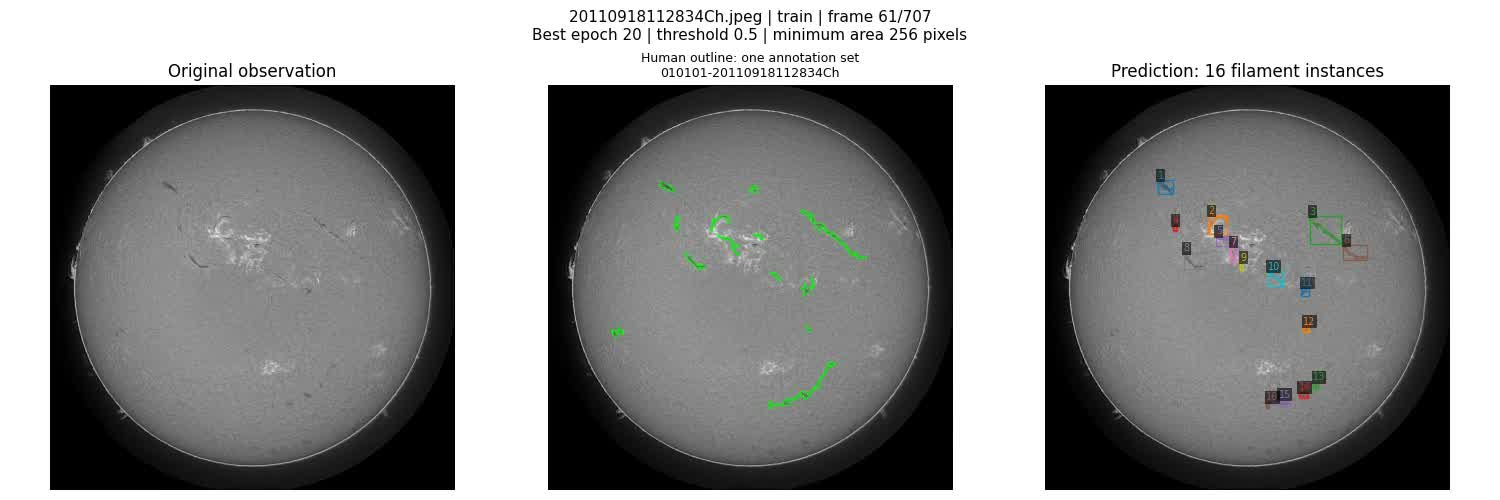
\includegraphics[width=\linewidth]{../baselinevideo/thumbnail.jpg}
 \caption{Frame from the downloaded baseline review video: observation,
 human annotation, and model overlay with component-derived boxes.
 The labeled sequence includes training images and is qualitative evidence,
 not an independent performance estimate. A one-minute looping preview
 is prepared for the repository README.}
 \label{fig:review}
\end{figure}

% ==================================== %
%              EVALUATION              %
% ==================================== %
\subsection{Baseline sampling and validation}
The first-version baseline uses one fixed observation-day-grouped
training/validation/holdout split, not $K$-fold cross-validation.
Observing days are shuffled with random seed 2026 and assigned approximately
70\%, 15\%, and 15\% to the three partitions, respectively; these proportions
apply to days, so image counts need not match them exactly. All observations
from the same day, including all annotator-specific targets for a physical
image, remain in one partition to reduce leakage between related observations.
Each annotator's filament masks are combined within that annotation set,
without merging labels across annotators.

The training partition is used for gradient updates. The validation
(tuning) partition determines the lowest-loss checkpoint and the
probability threshold and minimum component area used in post-processing.
The holdout partition provides a separate local evaluation, while the
unlabeled competition test set is used for inference and Kaggle scoring,
not local parameter selection.

\section{Evaluation}\label{sec:evaluation}
    \guide{Explain your evaluation. This includes:
    \begin{itemize}
        \item the evaluation strategy,
        \item plots and/or tables showing the performance of the segmentation algorithm (please include error bars and uncertainty measures whenever possible),
        \item strengths and weaknesses of the proposed algorithm, and possible strategies for improvement.
    \end{itemize}}

\subsection{First-version reporting status}
The baseline trained for 20 epochs. Saved training and validation time
was 2252.6 seconds (37.5 minutes) on a Tesla T4; this excludes downstream
calibration, inference, and rendering. Kaggle submission 58301531 completed
with public PQ of 0.29, verified through the API on November 13, 2026.
The CSV contained 1421 instances after processing 180 test images; three
zero-detection image omissions were accepted for this submission.
Local holdout PQ was 0.3350, Dice 0.6405, and IoU 0.4885 on 105 physical
images. These local and leaderboard figures use different evaluation data
and must not be interpreted as interchangeable estimates.

\subsection{Metrics and comparisons}
Local evaluation reports Panoptic Quality (PQ)~\cite{pq}, foreground
Dice, and intersection over union. PQ matches instances one-to-one
at intersection over union strictly greater than 0.5. Scores are averaged
across annotators within each physical image, then across images.
Local PQ is a diagnostic; equivalence to the competition evaluator has
not been established. Final leaderboard results must come from Kaggle.

\begin{table}[t]
\centering
\caption{Results placeholders. Dashes denote unmeasured values, not zero
performance. V1 and V2 use different evaluation protocols; their local
scores must not be interpreted as a paired ablation.}
\label{tab:pending}
\begin{tabular}{lccc}
\hline
Experiment & PQ & Dice & Kaggle PQ\\
\hline
V1: frozen 512 baseline & 0.3350 & 0.6405 & 0.29\\
V2: focused fine-tuning & --- & --- & 0.32\\
V3: YOLO + crop refinement, repaired & --- & --- & 0.35\\
V2: 512, raw & --- & --- & ---\\
V2: 512, CLAHE & --- & --- & ---\\
V2: 1024, raw & --- & --- & ---\\
V2: 1024, CLAHE & --- & --- & ---\\
V2: inner-selected procedure & --- & --- & ---\\
V2: fold-model ensemble & --- & --- & pending\\
\hline
\end{tabular}
\end{table}
V2 outer-fold values will be reported as mean $\pm$ sample standard
deviation only after all three folds finish, alongside executed epochs,
stopping reason, runtime, hardware, and completed-trial counts.
Missing or budget-truncated results will be disclosed, not imputed.
Outer-fold scores characterize individual fold models or the selection
procedure, not independent evaluation of the final fold-model ensemble.

\section{Version 2: Experimental Protocol}\label{sec:v2}
\subsection{Focused continuation experiment}
A separate focused experiment starts from the verified V1 checkpoint
with a fresh AdamW optimizer at learning rate $10^{-4}$ and batch size
two. It changes input resolution to 1024 pixels and applies CLAHE with
clip limit two and an $8\times8$ tile grid after resizing. It retains
the V1 training and tuning partitions, including the same calibration
image subset, and does not reevaluate holdout labels for selection.
Up to 40 additional epochs are permitted, with early stopping at patience
eight and significant-loss decrease $10^{-4}$, plus a plateau scheduler.
The inherited weights are evaluated at additional epoch zero under the
new preprocessing and retained if no later checkpoint improves tuning loss.
CUDA mixed precision is used for model operations with float32 loss
reductions. This is fine-tuning, not an optimizer-state resume.

The cooperative two-hour allowance reserves ten minutes for calibration
and test inference. V1 tuning loss decreased from 0.18129 at epoch 18
to 0.17807 at epoch 20, motivating further investigation but not proving
that insufficient epochs caused the leaderboard score. The experiment
changes several factors together and therefore cannot establish a causal
benefit from longer training, resolution, or CLAHE individually.
Kaggle submission 58304132 completed with public PQ of 0.32, verified
through the API on November 13, 2026. This is a 0.03 absolute increase
over V1, not evidence that any single changed factor caused the gain.
Grouped-fold controls below remain a separate study.

\subsection{Grouped-fold search}
The new notebook implements three observation-day-grouped outer folds.
Each outer training partition reserves approximately 20\% of its days
as an inner validation holdout. This uses inner holdout tuning, not an
additional inner $K$-fold loop. Fresh
ImageNet initialization is used for every candidate in every fold.
The distinction between parameter selection and outer evaluation addresses
selection bias~\cite{varma2006}. Previously inspected V1 holdout images are
not described as a new untouched final test set.

Four controls compare 512- and 1024-pixel inputs, with and without
CLAHE~\cite{opencvclahe}. CLAHE uses clip limit 2
and an $8\times8$ tile grid after resizing; the same transformation is used
in training and inference. These controls use learning rate
$3\times10^{-4}$, weight decay $10^{-2}$, and batch size two. Two additional
seeded random candidates at 1024 pixels with CLAHE sample learning rates
log-uniformly from $10^{-5}$ to $10^{-3}$. Weight decay is sampled
log-uniformly from $10^{-5}$ to $10^{-2}$. Batch size is two or four,
and clip limit is 1.5, 2, or 3. This follows random-search
methodology~\cite{bergstra2012}, without establishing a global optimum.

Each trial permits up to 60 epochs, with inner-loss early stopping
(patience eight, minimum significant decrease $10^{-4}$).
A plateau scheduler halves the learning rate after three non-improving
epochs. Checkpoints retain the strictly lowest inner loss.
Threshold candidates are 0.35, 0.5, and 0.65. Minimum area candidates
are 64 and 256 pixels at the original resolution.
Calibration uses up to 12 seeded inner validation images.
Candidate selection uses inner PQ only; outer labels do not determine
checkpoints, thresholds, or the selected candidate.

The default wall-time allowance for nested training and scoring is two
hours, configurable by researchers. Training receives 55\% of each
remaining job's equal time share, reserving the remainder for evaluation.
Checks occur between batches and images; individual operations and
installation/download/export overhead may exceed the allowance.
Eighteen trials of up to 60 epochs are unlikely to finish under this
budget. Time-truncated training is not evidence of convergence.
Longer-budget runs use a new experiment identifier; the notebook preserves
completed artifacts and explicitly marks incomplete folds.

\subsection{Hypotheses, not observed improvements}
\textbf{H1:} Higher resolution may retain thin structures lost during
downsampling and improve filament recall or PQ, at increased memory and
runtime cost. \textbf{H2:} CLAHE may expose faint structures but may also
amplify artifacts and increase false positives.
\textbf{H3:} Longer training with early stopping and a plateau scheduler
may improve validation performance if V1 is underfit, but may instead
overfit. A decreasing training loss alone does not establish improved
generalization or justify a particular epoch count.
The paired V2 controls will test these directional hypotheses; no
numerical gain or superiority claim is made before measurement.

The optional test export averages probabilities from the three selected
fold models at full resolution, using the median of their calibrated
thresholds and areas. This post-processing choice is a heuristic, not
separately optimized ensemble calibration. Test inference never selects
hyperparameters. The public reproducibility package must include the
selected weights, configuration, fold manifests, package versions,
calibration, and final report before the organizers' form is submitted.



\section{Version 3: Instance-Aware Experiment}
V3 replaces connected-component instance extraction from a semantic
foreground model with YOLO11s instance segmentation~\cite{ultralyticsseg}.
A separate U-Net with a ResNet18 encoder refines square crops around
detected instances. The working hypothesis is that explicit instance
proposals and local refinement may improve instance overlap and separation;
The repaired V3 submission achieved public PQ of 0.35, compared with
0.32 for focused V2 and 0.29 for V1. These exploratory runs change multiple
factors and do not isolate an architectural effect or establish parity
with a supplied reference notebook.

The detector uses 1024-pixel input, one filament class, up to 60 epochs,
and patience eight. All annotator label sets remain separate training
targets within the fixed observation-day split. The crop refiner uses
256-pixel crops with 1.8 times context, up to 20 epochs, Dice/BCE loss,
and lowest tuning-loss checkpoint selection. Training allowances are
75 minutes for the detector and 30 minutes for the refiner; preparation,
calibration, and inference add overhead.
Detector confidence, crop threshold, minimum area, and the choice between
YOLO-only and refined output are selected on the same tuning subset.
The initial V3 submission (58315901) was rejected for overlapping instance
masks and provides no valid leaderboard measurement. Offline repair of
the saved predictions, without retraining, produced submission 58316663;
its completed public PQ of 0.35 was verified through the Kaggle API.
The corrected pipeline assigns contested pixels to the earliest prediction
in proposal order and removes empty or below-minimum-area remnants.
This deterministic disjoint-mask policy is applied during both calibration
and export, with an independent zero-overlap validation. Previously saved
calibration metrics do not characterize the corrected predictions.

EDA plots connect grayscale histograms and spatial gradients to the
annotated images, illustrate resolution-dependent target sampling,
and follow normalized polygon coordinates through crop transformations.
Post-training review separates pixel errors from pairwise instance IoU
and PQ matching. Training crops use true instance bounds, whereas inference
crops use detector proposals: this mismatch and duplicate refinements are
limitations. The refiner cannot recover undetected instances.
An empty refinement falls back to its actual detector mask and is audited;
no mask is invented for an empty observation. V3 is a fixed-split
experiment, not grouped $K$-fold cross-validation.

% ==================================== %
%            ACKNOWLEDGMENT            %
% ==================================== %
\section{Acknowledgment}\label{sec:acknowledgment}
    % Do not change
    The organization of the Filament Segmentation Challenge 2026 is partially supported by the U.S. National Science Foundation (NSF) under Grant No. 2209912 and 2433781, directorate for Computer and Information Science and Engineering (CSE), and Office of Advanced Cyberinfrastructure (OAC), and Grant No. 2511630, AST Division Of Astronomical Sciences and MPS Directorate for Mathematical and Physical Sciences.

    The Filament Segmentation Challenge 2026 is sponsored by the U.S. National Science Foundation (NSF) National Solar Observatory (NSO).

    This work utilizes GONG data obtained by the NSO Integrated Synoptic Program, managed by the National Solar Observatory, which is operated by the Association of Universities for Research in Astronomy (AURA), Inc. under a cooperative agreement with the National Science Foundation and with contribution from the National Oceanic and Atmospheric Administration. The GONG network of instruments is hosted by the Big Bear Solar Observatory, High Altitude Observatory, Learmonth Solar Observatory, Udaipur Solar Observatory, Instituto de Astrofísica de Canarias, and Cerro Tololo Interamerican Observatory.

\bibliographystyle{ACM-Reference-Format}
\bibliography{main}

\end{document}
